\documentclass[12pt]{article}
\usepackage{graphics}
\newcounter{problem}
\begin{document}

\section*{Real Problems \\
          for NYU General Physics 1, Fall 2004}

\paragraph{\problemname~\theproblem}
\refstepcounter{problem}
\textsl{(a)}~What is the maximum amount of cash you can obtain by
successfully robbing an armored truck?  Assume that it is packed with
twenties; that is, estimate an answer by considering the volume of the
truck, and (harder to estimate) the volume of a 20-dollar bill.  State
your assumptions and explain your work, but please don't attempt an
experiment.  Be sure to explain exactly how you estimated the volume
of a 20-dollar bill.  \emph{Hint: think of a stack of bills to
  estimate the volume.  Feel free to \emph{check} any part of your
  answer on the internet, but make sure you actually make a justified,
  quantitative estimate independently.}

\textsl{(b)}~Do you think that many of the armored trucks in Manhattan
are fully packed with 20-dollar bills?

\textsl{(c)}~Would a similar truck weigh more, less, or about the same
if it contained the same amount of money but in the form of gold bars
instead of 20-dollar bills?

\paragraph{\problemname~\theproblem}
\refstepcounter{problem}

What is the mean acceleration $a$ of a dragster (ie, a drag-racing
automobile) that can travel 1/4~mi in 5.5~s, starting from a dead
stop?  Assume that the dragster accelerates with constant acceleration
throughout the 5.5~s (not a terrible assumption, but not a good one
either).  Give your answer in terms of the gravitational acceleration
$g$.  Does your answer seem reasonable?  What do you predict, under
the constant-acceleration assumption, for the final speed
$v_\mathrm{f}$ of the dragster as it crosses the finish line?  Give
your answer in $\mathrm{mi\,h^{-1}}$.  Search the WWW for the current
world-record 1/4~mi drag-race time and final speed.

\paragraph{Problem~\theproblem:}\refstepcounter{problem}%
A bit on air resistance and terminal velocities. If you want more
discussion of these issues, see \url{http://arxiv.org/abs/0709.0107}
(click the PDF link at the right of the page).

\textsl{(a)}~Show that the ram-pressure-force formula $\rho\,A\,v^2$ has the
correct units to be a force, when $\rho$ is a mass density, $A$ is a
cross-sectional area, and $v$ is a speed. Look up air drag on
Wikipedia and see what this formula is missing.

\textsl{(b)}~At what downward falling speed $v$ does an object with
mass $M$ and cross-sectional area $A$ find that ram pressure balances
the gravitational force? Derive an expression. This is the formula
(ish) for the terminal velocity!

\textsl{(c)}~Two pennies are dropped (carefully) from a tall building,
one so that it falls precisely edge-on, and one so that it falls
precisely face-on (difficult but not impossible in practice).  What
(roughly) are the two terminal velocities and what (roughly) is
their ratio $v_{\mathrm{edge}}/v_{\mathrm{face}}$?

\textsl{(d)}~Roughly how far does a typical American car have to drive
to ``sweep up'' or drive through a column of air that is comparable in
weight to the car itself?  You will have to estimate the
cross-sectional area and weight of a typical car (or look both things
up on the web; if you look them up, give the make and model).

\textsl{(e)}~Describe in words the \emph{environmental significance}
of the distance you calculated in part \textsl{(d)} of the previous
problem.

\paragraph{\problemname~\theproblem}
\refstepcounter{problem}

\textsl{(a)}~Imagine a stone thrown upwards at $5~\mathrm{m\,s^{-1}}$.
How far does it travel in the first 0.1~s after the throw?
Approximate its velocity as being constant during that 0.1~s interval.

\textsl{(b)}~In a coordinate system in which the $x$ direction points
upwards, the stone's $x$-direction velocity $v_x(t)$ is given
(approximately) by
\begin{equation}
v_x(t)= [5~\mathrm{m\,s^{-1}}]-[10~\mathrm{m\,s^{-2}}]\,t \quad ,
\label{eq:stone_velocity}
\end{equation}
where $t$ is the time since the throw (implicitly, the throw was at
$t=0$).  What is the new velocity of the stone at time
$t=0.1~\mathrm{s}$, and how far does it travel in the \emph{next}
0.1~s of its travel?  Again, approximate the velocity as being
constant during the interval.

\textsl{(c)}~Now make a table of times, 0.0~s, 0.1~s, 0.2~s, etc, all
the way to 1.5~s.  At each time, compute the velocity of the stone,
using equation (\ref{eq:stone_velocity}), and compute the
$x$-direction displacement $\Delta x$ traveled in that interval.  Sum
up the intervals to get the total displacement $x$ traveled, starting
at $x=0$ at time $t=0$.  Approximate the velocity as being constant in
each interval.  Be sure to maintain the \emph{signs} of the
displacements; sometimes the stone will be rising and sometimes it
will be falling!

\textsl{(d)}~When, according to your chart, does the stone return to
$x=0$?  Does your answer agree, roughly, with an exact calculation?
Explain any discrepancy.

\paragraph{\problemname~\theproblem}
\refstepcounter{problem}

Lifting strength---measured in units of force---is roughly
proportional to the cross-sectional area of your legs (or arms).  Now
imagine that you have a near-identical twin, who is incredibly similar
to you except 1 percent smaller in every linear dimension.  By what
factor $f_s$ will her or his lifting strength differ from yours?  Who
can lift more?  By what factor $f_w$ will her or his weight differ
from yours?  Who can lift a greater fraction of her or his own weight?
Ants can lift objects much heavier than themselves.  Do your answers
shed light on this ``amazing'' fact?

\paragraph{\problemname~\theproblem}
\refstepcounter{problem}

If you stand on the equator of the Earth, you are not really standing
still but rather rotating around the center of the Earth once every 24
hours.  What is the magnitude of the centripetal acceleration
$a_\mathrm{c}$ associated with this rotation?  Give your answer as a
fraction of the gravitational acceleration $g$.

\paragraph{\problemname~\theproblem}
\refstepcounter{problem}

Draw, on graph paper, the curves of one-dimensional acceleration $a_x$
and position $x$, corresponding to this curve of a particle's velocity
$v_x$:
\\ \rule{0.1\textwidth}{0pt}
\resizebox{0.8\textwidth}{!}{\includegraphics{../pro/velocity_time.eps}}
\\
Assume that the particle begins at position $x=0$ at time $t=0$.  Make
your figures as quantitatively accurate as you can, and be sure to
clearly specify and label the axes of your two plots.

\paragraph{Problem~\theproblem:}\refstepcounter{problem}%
In a 200-m race, the winner crosses the halfway mark (ie, 100~m) at
$t_{1/2}=10.12$~s and the finish line at $t_{\rm f}=19.32$~s.  If you
make a kinematic model of the runner's behavior as (i)~constant
acceleration $a$ from rest for the period $0<t<t_a$ followed by
(ii)~constant speed $v=a\,t_a$ during the period $t_a<t<t_{\rm f}$,
what are $a$ and $t_a$?

\emph{Hint: Draw a graph of $v(t)$ before you start writing equations.}

\emph{Hint: Once you have a graph, consider the question: is $t_a$
going to be before or after $t_{1/2}$?  Make a quantitative argument.}

\emph{Hint: You can solve this problem with geometry and the graph; no
  need to do calculus!}

\paragraph{\problemname~\theproblem}
\refstepcounter{problem}

If you apply the brakes strongly, about how quickly can you stop a
typical automobile travelling at $60~\mathrm{mi\,h^{-1}}$?  Give an
answer in seconds.  If you don't drive, talk to someone who does.  The
automobile stops by applying a horizontal frictional force to the
ground.  Estimate the magnitude of the total frictional force $F_f$
required by this stop.  Give your answer both in Newtons and in
pounds.  You will have to estimate the mass of a typical automobile.
What is the direction of the frictional force applied by the
automobile to the ground?  What is the direction of the force applied
by the ground to the automobile?  Compute also the stopping distance,
ie, the distance traveled during the deceleration.  Give your answer
in meters.

\paragraph{\problemname~\theproblem}
\refstepcounter{problem}

The sine and cosine functions can be defined \emph{completely} by the
four constraints
\begin{equation}
\sin 0=0 \quad ;\quad
\cos 0=1 \quad ;\quad
\frac{\mathrm{d}\sin\theta}{\mathrm{d}\theta}=\cos\theta \quad ;\quad
\frac{\mathrm{d}\cos\theta}{\mathrm{d}\theta}=-\sin\theta \quad .
\nonumber
\end{equation}
We are going to approximate these equations with a chart like the one
we made for \problemname Set~1.

\textsl{(a)}~Compute approximate values for $\sin (0.1~\mathrm{rad})$
and $\cos (0.1~\mathrm{rad})$ by starting with the initial conditions
given above, approximating the derivative of $\sin$ to be constant and
equal to $\cos (0)$, and approximating the derivative of $\cos$ to be
constant and equal to $-\sin (0)$.

\textsl{(b)}~Compute approximate values for $\sin (0.2~\mathrm{rad})$
and $\cos (0.2~\mathrm{rad})$ by starting with what you computed in
part~(a), approximating the derivative of $\sin$ to be constant and
equal to the $\cos (0.1~\mathrm{rad})$ that you computed in part~(a),
and approximating the derivative of $\cos$ to be constant and equal to
the $-\sin (0.1~\mathrm{rad})$ you also computed in part~(a).  Do not
use your calculator!

\textsl{(c)}~Continue the above, computing, approximately, $\sin$ and
$\cos$, on a grid of angles 0.1, 0.2, 0.3, \ldots, $2.0~\mathrm{rad}$.
You may use a calculator, but you must not ever use either the
\fbox{$\sin$} button nor the \fbox{$\cos$} button.

\textsl{(d)}~Obtain an approximate value for $\pi/2$ by linearly
interpolating to the point at which your approximation of $\cos$
crosses zero.  Explain any discrepancy you get from the true value.
Suggest two ways you could you have improved your calculation.

\paragraph{\problemname~\theproblem}
\refstepcounter{problem}

Imagine a hypothetical package delivery system that involves launching
packages horizontally so fast that they travel on circular orbits just
skimming above the Earth's surface.  Imagine that the system operates
in evacuated tunnels, so air resistance can be ignored.  How fast $v$
does a package of mass $M$ have to be launched horizontally so that
the gravitational force $F_g$ on the package is just sufficient to
keep it on a uniform, circular orbit, with the center of the Earth at
the center of the orbit?  Give your answer in terms of the radius of
the Earth $R_E$, the acceleration due to gravity $g$, and anything
else you need.  How long $T$ does it take for the package to do a
complete orbit?  Again, give a symbolic expression.  When you are
done, plug in numbers and compare with the orbital period of the Space
Shuttle (look it up on the \textsc{www}).  Did you expect the period
of the Space Shuttle be more similar or more different from the period
of the package, or does it seem about right?

\paragraph{Problem~\theproblem:}\refstepcounter{problem}%
Imagine a package of mass $M$ sitting on the floor of an elevator that
is accelerating upwards at acceleration $a$. The acceleration due to
gravity is $g$.

\textsl{(a)} Draw the free-body diagram for the package.

\textsl{(b)} What is the magnitude $N$ of the normal force on the
package?

\textsl{(c)} Answer those same two questions again, but with the
elevator accelerating \emph{downwards} at acceleration $a$.

\textsl{(d)} Answer those same two questions again, but with the
elevator accelerating downwards at acceleration $g$ (that is, at
the gravitational acceleration).

\textsl{(e)} In lecture Prof Hogg did a stunt with a coffee cup and a
quarter. Draw the free-body diagram for the quarter when it was at the
top of the arc (that is, when it was directly overhead).

\paragraph{\problemname~\theproblem}
\refstepcounter{problem}

Explain why the astronauts in the Space Shuttle are ``weightless''.
Is it because there is no gravitational force in outer space?  No, it
certainly is not!

\paragraph{\problemname~\theproblem}
\refstepcounter{problem}

Why is it that flying airplanes must bank (ie, tilt) to turn?  Why
can't they simply turn horizontally like an automobile can?

\paragraph{\problemname~\theproblem}
\refstepcounter{problem}

Imagine that a typical power line in the countryside is made of copper
wire of about 0.5~cm diameter, stretched horizontally from telephone
pole to telephone pole, with the poles separated by about 30~m.  The
wire sags by about 10~deg below the horizontal where it is attached to
each pole (because the wire is pulled down by gravity).  What is the
approximate tension $T$ in the wire?  You will need to know the
density of copper.  Draw a free-body diagram for one 30-m segment of
the wire.  Clearly state any simplifying assumptions you choose to
make.

\paragraph{\problemname~\theproblem}
\refstepcounter{problem}

A thin, uniform beam of mass $m_\mathrm{b}$ and length $L_x$ is
attached to a wall by a pivot and a wire, as shown.  The beam supports
a sign of mass $m_\mathrm{s}$.
\\ \rule{0.35\textwidth}{0pt}
\resizebox{0.3\textwidth}{!}{\includegraphics{../mp/hanging_sign.eps}}
\\
Find the tensions $T_1$ and $T_2$ in the two wires and the vector
force $\vec{F}$ on the beam at the pivot, in terms of the quantities
shown and the acceleration $g$ due to gravity.  Assume that the pivot
is frictionless (so it provides no torque) and that the wires are
massless.  If there was friction on the pivot, what parts of your
answer would change, and in which direction?

\paragraph{\problemname~\theproblem}
\refstepcounter{problem}

To a good approximation, the air resistance force $F_\mathrm{air}$
acting on a moving car can be computed simply from the density $\rho$
(mass per volume) of air, the speed $v$ of the car, and the
cross-sectional area $A$ of the car.  Use a dimensional argument to
estimate the air resistance force (in Newtons) acting on a typical car
driving at $55~\mathrm{mi\,hr^{-1}}$.  You will need to say what you
are assuming for the density of air $\rho$ and the cross-sectional
area $A$ of the car.  Reasonable estimates are preferred to
unreasonable ones!

\paragraph{\problemname~\theproblem}
\refstepcounter{problem}

Calculate the force $F$ at which the machine illustrated below can be
pulled such that mass $m_2$ neither falls nor rises.  All surfaces are
frictionless.
\\ \rule{0.2\textwidth}{0pt}
\resizebox{0.6\textwidth}{!}{\includegraphics{../mp/pedagogical.eps}}

\emph{Hint: Draw all free body diagrams and work out all kinematic
relationships before trying to solve anything!}

\paragraph{Problem~\theproblem:}\refstepcounter{problem}%
NYC had a hot summer in 2016, with most buildings running air
conditioning on a thermostat continuously. To save energy, NYU asked
their employees to conserve energy in various ways, some of which we
might take issue with. Here's an uncontroversial one: You should take
the stairs, not the elevator.

\emph{But is that uncontroversial?}  In the parts that follow, make
sure you are explicit about your assumptions, and that your
assumptions are reasonable. If you are concerned with reasonableness,
do some experiments and make some observations.

\textsl{(a)} How much potential energy does a typical NYU employee
generate if he or she climbs 10 stories of stairs?

\textsl{(b)} How fast does a healthy, young (say 30s), typically abled
NYU employee climb this many stairs?

\textsl{(c)} Compare the kinetic energy of the employee while climbing
to the potential energy gain. Which dominates our considerations?

\textsl{(d)} What is the average horsepower mechanical output of this
NYU employee steadily climbing stairs? Why do you not need to consider
the kinetic energy \emph{at all} in this part, and that ignoring it
isn't even an approximation?

\textsl{(e)} For every kcal (look up the calorie and the kcal; what
are called ``calories'' in nutrition are actually kcal) of mechanical
energy generated, a healthy, fit human also generates about 7 times
more in metabolic load; that is, you burn some 8 times your
mechanically computed power in food calories. How many kcal did the
employee burn going up the 10 stories?

\textsl{(f)} Now imagine (correctly) that all that metabolic energy
gets dumped into the building atmosphere and needs to get corrected by
the building air conditioning. Air-conditioning units are very
inefficient; they produce multiple BTU (or kcal or J or kWh) of heat
for every BTU (or kcal or J or kWh) of cooling they do. Look up
efficiencies for typical AC systems and figure out what load an
employee puts on the AC by climbing this far.

\textsl{(g)} [Not for credit!] For \emph{extremely deep reasons}, an
elevator can't be perfectly efficient either. Can you think of some of
these reasons? Prof Hogg knows at least three unbeatable physical
constraints. The relevant question for us is: Does an elevator burn
more than eight times the mechanical work it is doing, and does it
drop that load inside the building AC system? If you want, do some
research to understand this. The ``nicest'' assumption you can make
about the elevators is that they are always crowded, so you are only
looking at the \emph{marginal} cost of bringing up one more person.

\paragraph{Problem~\theproblem:}\refstepcounter{problem}%
Gasoline and olive oil are both substances with great chemical energy
content per unit mass.

\textsl{(a)} In the case of gasoline, the chemical energy is mainly in
carbon bonds.  If you assume that gasoline is \emph{entirely} carbon
atoms, and each one releases $4\,\eV$ of energy when it is combusted, how
much energy per unit mass is there in gasoline?  Get an answer in MJ
per kg and compare to what you find on \textit{Wikipedia}.  How far off
are our assumptions?

\textsl{(b)} Now convert your answer to kcal per g and compare it to
what is written on the ``Nutrition Facts'' label on an olive oil
bottle.  How close are you?  It should be close, (Prof Hogg thinks), because
biofuel is made from things like olive oil!

\textsl{(c)} Now assume that a car moving at speed
$v=75\,\mi\,\h^{-1}$ encounters an air resistance force of
$\rho\,A\,v^2$, where $\rho$ is the density of air and $A$ is the
cross-sectional area of the car, about $2.5\,\m^2$ How much work does it
take to move the car $30\,\mi$ at this speed?

\textsl{(d)} If a car with these properties was \emph{perfectly
  efficient}, how many miles per gallon would it get?  What does this
make you think about the future of cars that are \emph{far more
  efficient} than cars we have today?

\paragraph{Problem~\theproblem:}\refstepcounter{problem}%
Here is a non-trivial machine that delivers a kind of mechanical
advantage:
\\ \rule{0.33\textwidth}{0pt}
\resizebox{0.33\textwidth}{!}{\includegraphics{../mp/tackle_blocks.pdf}}

\textsl{(a)}~Draw free-body diagrams for all the masses and pulleys in
this mechanism. Assume that the strings and pulleys are light and
frictionless, so that the strings are perfect tension-transmitters.

\textsl{(b)} What is the kinematic constraint---the relationship
between the accelerations of block 1 and block 2? Be very careful with
this one. Treat all the strings as inextensible for simplicity.

\textsl{(c)} Find the tensions in all three strings and the
accelerations of the two blocks.

\textsl{(d)}~Now set the mass $m_2$ to the value it must have if the
system is to be perfectly ``balanced''; that is, for there to be no
net acceleration of either block.  In this situation, if block $m_1$
is lowered a small distance $h$, what is the net change in potential
energy, accounting for the displacements of both blocks?

\paragraph{\problemname~\theproblem}
\refstepcounter{problem}

Two blocks of mass $M$ are placed on an inclined plane, inclined at an
angle $\theta$ to the horizontal.  One has a small coefficient of
sliding friction $\mu_\mathrm{k}$ that is insufficient to keep it from
accelerating down the plane.  Compute the magnitude of the frictional
force $f_\mathrm{k}$ and the magnitude of the block's acceleration
$a$.  The other block has a large coefficient of static friction
$\mu_\mathrm{s}$ that is sufficient to keep it from sliding.  Compute
the magnitude of the frictional force $f_\mathrm{s}$ acting on this
static block.  If your answer is correct, the coefficient
$\mu_\mathrm{s}$ does not appear in the expression.  Explain why not.

\paragraph{\problemname~\theproblem}
\refstepcounter{problem}

A typical American car gets about $25~\mathrm{mi\,gal^{-1}}$, driving
at a constant speed of $55~\mathrm{mi\,h^{-1}}$ on level ground.
Since the car is neither climbing nor accelerating, the power put out
by the motor is simply fighting friction and air resistance (drag).
Use these two facts to derive the total force (friction plus drag)
against which the motor is acting.  Give your answer in Newtons.
Useful facts include: (1)~the molecular weight of gasoline is roughly
$100~\mathrm{amu}$ (ie, a typical gasoline molecule is about 100 times
the mass of a hydrogen atom); (2)~gasoline is slightly less dense than
water (but not far less dense); (3)~the typical amount of energy
released when a single gasoline molecule is burned is a few eV, or,
say $5\times 10^{-19}~\mathrm{J}$; and (4)~a typical car is probably
only about 25~percent efficient in its conversion of chemical energy
into mechanical energy.  Compute the mechanical power being exerted
against friction and drag at $55~\mathrm{mi\,h^{-1}}$ in horsepower
(you might have to look up the conversion on the WWW).  Compare that
horsepower to the rated horsepower of some typical American cars.
Does your answer seem reasonable?

\paragraph{\problemname~\theproblem}
\refstepcounter{problem}

A turn in a road, with a radius of curvature $R=150~\mathrm{m}$, is
banked at an angle $\theta$, optimized for travel at
$55~\mathrm{mi\,h^{-1}}$.  What is that angle $\theta$?  Now imagine
that on a rainy day the coefficient of static friction between a car's
tires and the road is 0.5.  What is the maximum speed $v_\mathrm{max}$
at which the car can take the turn?  Be sure to draw a very clear
free-body diagram for the car.

\paragraph{\problemname~\theproblem}
\refstepcounter{problem}

Give estimated values (in SI units) for (a)~the kinetic energies, and
(b)~the momenta of: (1)~a bullet fired from a rifle, (2)~a soccer ball
kicked hard, and (3)~a three-year-old riding slowly on a tricycle.
You will have to make estimates of the masses and speeds of all three.
Clearly state your assumptions and estimates.

\paragraph{Problem~\theproblem:}\refstepcounter{problem}%
A student of mass $m_\mathrm{student}=80\,\kg$ stands at rest next to
a block of ice of mass $m_\mathrm{ice}=320\,\kg$, also at rest, on a
frictionless frozen lake.  The student pushes on the block until the
block is moving away from the student at $1.5\,\mps$ (that is, until
$\left|\vec{v}_\mathrm{ice}-\vec{v}_\mathrm{student}\right|=1.5\,\mps$).
How much work did the student do?  Give your answer in $\J$.  Don't
forget to conserve linear momentum!  \emph{Hint:} All that work went into
kinetic energy.  \emph{Another hint:} One of the hard things about
this problem is that I am giving you the \emph{relative} velocity and
not the absolute velocity.  How are you going to deal with that?
Spend some time visualizing the problem before writing equations.

\paragraph{\problemname~\theproblem}
\refstepcounter{problem}

A block of mass $5~\mathrm{kg}$ moving initially at speed
$7~\mathrm{m\,s^{-1}}$ in the positive $x$ direction collides
elastically with another block of mass $2~\mathrm{kg}$ moving
initially at speed $2~\mathrm{m\,s^{-1}}$ in the negative $x$
direction.  If the blocks recoil in the $x$ direction (ie, if the
problem remains one-dimensional), what are the final velocities of the
blocks?  Assume that there is no friction, drag or any other external
force.

\paragraph{Problem~\theproblem:}\refstepcounter{problem}%
A machine at a packaging facility places stationary packages of mass
$m$ onto a horizontal conveyor belt that is moving packages steadily
and horizontally at speed $v$. Once placed on the belt, the packages
start moving at speed $v$; that is, they are rapidly accelerated.

\textsl{(a)} What is the momentum change for each package as it
gets placed on to the belt, and what is the kinetic energy change?

\textsl{(b)} Imagine that the machine places packages steadily onto
the belt, with time intervals $T$ between packages. Compute the
average mechanical power required by the belt by dividing the kinetic
energy per package by the time interval between packages.

\textsl{(c)} Now compute the average force the belt is applying to the
packages by dividing the momentum per package by the time interval
between packages. This is possible, because momentum is force per unit
time (if that is a surprise, do some library or web research).

\textsl{(d)} Power is force times velocity (dot product, really); so
the force answer can be turned into a power answer and compared to the
power you computed above.

\textsl{(e)} Do you have a discrepancy? If so, why? Which answer is
more correct?

\paragraph{\problemname~\theproblem}
\refstepcounter{problem}

\textsl{(a)} A bullet of mass $m$ initially traveling in the $x$
direction at high speed $v$ hits and imbeds itself in a block of mass
$M$ initially at rest.  What is the final speed $v'$ of the block,
now of mass $M+m$?  How much kinetic energy $\Delta K$ was lost in the
collision, if any?

\textsl{(b)} If the block was initially hanging from the ceiling by a
very light, long, inextensible string of length $\ell$, to what height
$\Delta h$ does the block rise (swing up) after the collision?

\textsl{(c)} Explain, very concisely, why you solved part (a) with
conservation of momentum, and part (c) with conservation of energy,
and not the other way around.

\textsl{(d)} Explain, very consisely, why you were allowed to treat
the collision part of the problem separately from the swinging part of
the problem.  Why can you approximate the collision as being finished
before it starts to swing?  \textit{Hint: Try comparing timescales.}

\paragraph{\problemname~\theproblem}\refstepcounter{problem}\label{elastic}
...placeholder...

\paragraph{\problemname~\theproblem}\refstepcounter{problem}

Re-do \problemname~\ref{elastic}, but now for the left-hand block having
mass $M$ and the right-hand block having mass $m\ll M$; that is, solve
the extreme mass-ratio problem. For initial velocities, use $v$ for
the big block and $0$ for the small block. Then draw the before and
after pictures in the lab and center-of-mass frames, just as you did
in \problemname~\ref{elastic}.

\paragraph{\problemname~\theproblem}
\refstepcounter{problem}

In a gas of (absolute) temperature $T$, the average-square speeds
$\left<v_x^2\right>$, $\left<v_y^2\right>$, and $\left<v_z^2\right>$
in the $x$, $y$, and $z$ directions are each roughly given by
\begin{equation}
\frac{1}{2}\,m\,\left<v_x^2\right> =
\frac{1}{2}\,m\,\left<v_y^2\right> =
\frac{1}{2}\,m\,\left<v_z^2\right> =
\frac{1}{2}\,k\,T \nonumber \;\;\; ,
\end{equation}
where $k$ is Boltzmann's constant.  Air is primarily made up of
$\mathrm{N_2}$ gas.  What is the typical speed of an air molecule at
room temperature?  How does it compare to the speed of sound?  What is
the typical magnitude of the impulse $\Delta\vec{p}$ of a collision of
a $\mathrm{N_2}$ molecule with your hand?  If your hand is feeling
$15~\mathrm{lb\,in^{-2}}$ of pressure, how many molecules, roughly,
are hitting your hand every second?

\textit{You will have to look up $k$, the mass of a $N_2$ molecule (or
a N atom), the absolute temperature $T$ of room temperature, and the
speed of sound.  The rest you should calculate, and show your work.
Your answers need not be precise!}

\paragraph{\problemname~\theproblem}
\refstepcounter{problem}

You can model the force of the wind on a sailboat's sail as being from
elastic collisions of air molecules against the surface of the sail.
Treat the air molecules as all having the same momentum $\vec{p}_i$
and the sail as a perfectly flat surface of area $A$ with normal
vector $\hat{n}$.

\textsl{(a)} Show that the number of molecules of air hitting the sail
per unit time is proportional to the cosine of the angle $\theta$
between the normal vector $\hat{n}$ and the wind momentum $\vec{p}_i$.
Check your answer for $\theta=0$ and $\theta=\pi/2$.

\textsl{(b)} Show that the impulse $\Delta\vec{p}$ of each air
molecule collision is also proportional in magnitude to $\cos\theta$,
and that the direction of $\Delta\vec{p}$ is normal to the sail
surface.
\\ \rule{0.3\textwidth}{0pt}
\resizebox{0.4\textwidth}{!}{\includegraphics{../mp/sailboat.eps}}

\textsl{(c)} Imagine that the sailboat is trying to sail at an angle
$\beta=90~\mathrm{deg}$ with respect to the wind direction.  What is
the best angle $\theta$ at which the sailors ought to set the sail?
Assume that the sailors want to maximize the component of the force
from the sail that is in the direction of the motion of the boat.

\paragraph{\problemname~\theproblem}
\refstepcounter{problem}

In Problem Set 3 you computed the speed of a package delivery system
involving packages on orbits around the Earth.  Imagine that the
packages are launched using rockets that expel their propellant at
about the speed of sound (relative to the rocket).  What must be the
ratio of the mass of propellant to the mass of the package in order
for the rockets to get the packages onto their correct orbits?  If the
propellant costs the same amount per pound as gasoline, how much would
it cost to get your textbook onto the orbit?  Compare this to the
price of an overnight delivery service.  Why is the speed of sound the
relevant speed for the propellant?  Do you expect the speed of sound
in rocket propellant (which is hot) to be higher or lower than the
speed of sound in normal air?  If your rocket can expel its exhaust at
ten times the speed of sound, by how much does that reduce or increase
your costs?

\paragraph{\problemname~\theproblem}
\refstepcounter{problem}

Compute the angular momentum $L_\mathrm{orbit}$ of the Earth's orbital
motion around the Sun.  Treat the Earth as a point particle on a
circular orbit.  Compute the angular momentum $L_\mathrm{spin}$ of the
Earth's spin.  Treat the Earth as a uniform sphere spinning in place
once per day.  You will have to look up the moment of inertia $I$ of a
uniform sphere, and maybe some Solar System data.  Give your answers
in SI units and also give the ratio
$L_\mathrm{spin}/L_\mathrm{orbit}$.  Also compute the kinetic energies
of the spin and orbital motions.  Again, give your answers in SI units
and also give the ratio.

\paragraph{\problemname~\theproblem}
\refstepcounter{problem}

In a pool shot, the cue ball (mass $m$), moving initially with
momentum $\vec{p}_\mathrm{ci}$, hits the five ball (also mass $m$),
initially at rest.  After the elastic collision, the five ball moves
at momentum $\vec{p}_\mathrm{5f}$, at an angle $\theta$ to the cue
ball's initial momentum vector.  The cue ball recoils with momentum
$\vec{p}_\mathrm{cf}$.

Draw a vector diagram showing the three momenta.  Use conservation of
momentum, conservation of energy, and geometry to show that the final
momenta $\vec{p}_\mathrm{5f}$ and $\vec{p}_\mathrm{cf}$ are
perpendicular.  You might use the fact that $KE= p^2/(2m)$.

\emph{Note that the final momenta are only perpendicular in the
particular case of equal masses.}

\paragraph{\problemname~\theproblem}
\refstepcounter{problem}

Why were you allowed to ignore friction during the pool shot in the
previous Problem?  \emph{Consider the magnitudes of the forces, or the
work they do through the duration of the impact.}

\paragraph{\problemname~\theproblem}
\refstepcounter{problem}

A heavy round pipe of mass $m$, radius $R$, and moment of inertia $I$
sits at rest on the horizontal bed of a parked truck, a distance $L$
from the end of the truck bed.  At time $t=0$, the truck starts to
accelerate forwards with acceleration $a$, at which point the pipe
begins to roll without slipping on the truck bed.  Give all your
answers with respect to the stationary ground, {\em not} the moving
truck.
\\ \rule{0.3\textwidth}{0pt}
\resizebox{0.4\textwidth}{!}{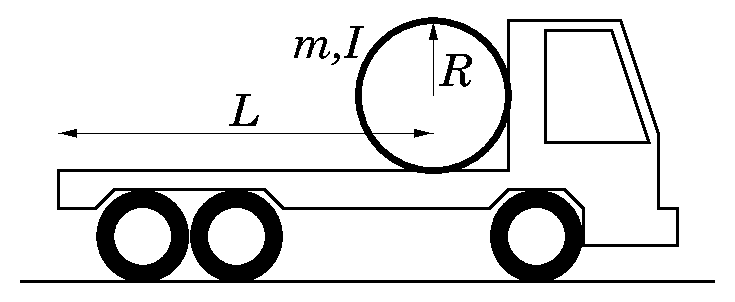
\includegraphics{../eps/truckpipe.eps}}

\textsl{(a)} During the acceleration, when the truck is moving at
speed $v_t$ and the pipe is moving at speed $v_p$ (with respect to the
ground) and the pipe is spinning at angular speed $\omega_p$, what is
the condition (ie, equation relating $v_t$, $v_p$, $\omega_p$ and $R$)
for rolling without slipping on the truck bed?

\textsl{(b)} Draw a free body diagram for the pipe, showing all
forces, for $t>0$.

\textsl{(c)} At what time $t_f$ does the pipe fall off the back of the
truck?

\emph{Do not solve this problem with pseudo-forces; your equations and
free-body diagrams should only show real forces (such as gravity,
friction, normal forces, etc.).}

\paragraph{\problemname~\theproblem}
\refstepcounter{problem}

\textsl{(a)} A typical golfer can hit a golf ball about 300 yards.
Under the assumption that you can ignore air resistance, estimate the
speed at which the club head is moving just before it strikes the
ball.  Assume that the club head is ten times as massive as the ball.

\textsl{(b)} Now check your assumption about air resistance by
figuring that the air is (on average) ``at rest'' with respect to the
ground, that the air is made up primarily of $\mathrm{N}_2$ molecules,
and that air molecules collide elastically with the ball during its
trajectory.  Compare the very approximate force you calculate with the
force due to gravity.  Note that this is \emph{not} a realistic model
for the force of air resistance, but it is also not insane.

\textsl{(c)} Now, against logic, assume that the ball's trajectory
follows the no-air calculation.  How much work is done by the ball on
the air?  Compare that work to the ball's initial kinetic energy.

\textsl{(d)} Was it reasonable to assume no air resistance?

\paragraph{\problemname~\theproblem}
\refstepcounter{problem}

\textsl{(a)}~A hockey puck (a uniform disk of mass $m$, radius $r$,
and thickness $t$), slides without friction on ice with initial speed
$v_0$.  It strikes an identical puck tangentially, as shown in the
figure, and sticks to it.  The second puck is initially at rest and
also can slide without friction.  What is the final (linear) velocity
(speed $v$ and direction) of the stuck-together pucks?  What is the
moment of inertia $I_f$ and final angular speed of rotation $\omega$
of the system around its center of mass?  What fraction of the initial
kinetic energy (if any) is lost; \textit{ie,} what is $[K_i-K_f]/K_i$?
\\ \rule{0.25\textwidth}{0pt}
\resizebox{0.50\textwidth}{!}{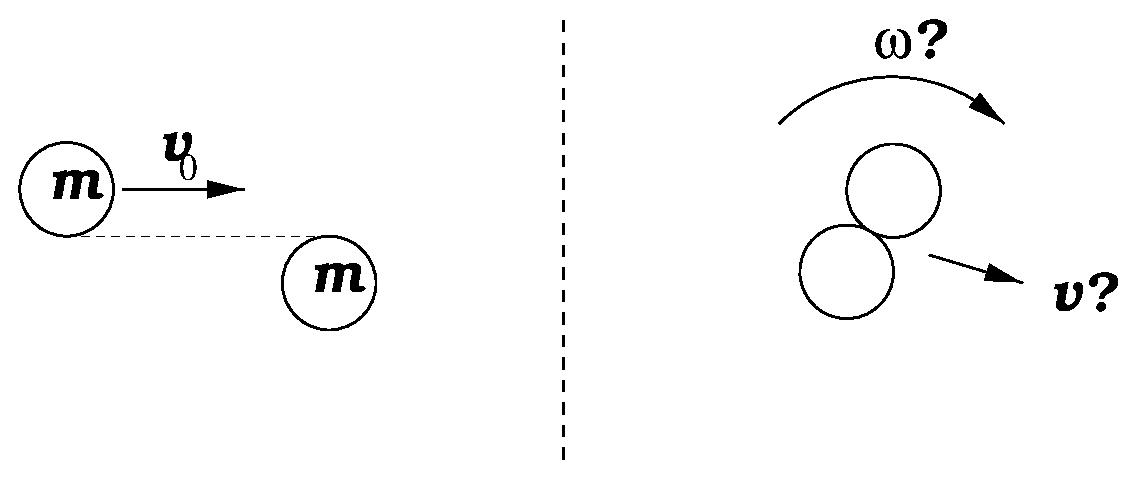
\includegraphics{../eps/tangpucks.eps}}
\\

\emph{Draw a clear diagram with a clearly labeled reference point used
to compute the angular momentum; recall that any angular momentum
calculation is with respect to your chosen origin.}

\textsl{(b)}~If the pucks had hit dead-on, the stuck-together pucks,
after the collision, would not be rotating.  Which of your answers
($v$, $\omega$, and $[K_i-K_f]/K_i$) will be different in this case?
If the fractional loss in kinetic energy is different, explain where
the difference in energy went.

% could ask about a pre-spinning incoming puck

\paragraph{\problemname~\theproblem}
\refstepcounter{problem}

\textsl{(a)}~Immediately after being hit, at $t=0$, a cue ball of mass
$M$ and radius $R$ slides along the felt at speed $v_i$, not rotating
at all.  As time goes on, the ball slows down (because of friction)
and, at the same time, starts to spin.  Draw a free-body diagram for
the cue ball.  At what time $t_\mathrm{r}$ does the ball get to the
situation of ``rolling without slipping''?  Assume that there is a
coefficient $\mu$ of sliding friction.

\textsl{(b)}~Plot $v(t)$ and $R\,\omega(t)$ vs $t$ on a single plot.
\emph{Note that the two things I have asked you to plot have the same
dimensions.}  Clearly label $t_\mathrm{r}$ on your diagram.

\paragraph{\problemname~\theproblem}
\refstepcounter{problem}

\textsl{(a)}~A figure skater spins in place on frictionless ice at
angular speed $\omega_i$ with her hands outstretched.  She has a total
moment of inertia $I_i$.  As the skater draws her hands into her body,
her moment of inertia decreases to $I_f=I_i/2$.  Does her kinetic
energy $K$ increase, decrease, or stay the same?  If it increases,
where does the energy come from?  If it decreases, where does the
energy go to?  \emph{Explain all your answers concisely but clearly:
What is conserved?}

\textsl{(b)}~Now estimate the moments of inertia: $I_i$ of an ice
skater with her hands outstretched, and $I_f$ of an ice skater with
her hands drawn in.  Is the factor of 2 used in part \textsl{(a)}
reasonable?

\paragraph{\problemname~\theproblem}
\refstepcounter{problem}

In Problem 2, above, how much heat energy is generated during the
slide?  Note that the answer is not the frictional force times the
distance traveled during the slide.  Why not; \textit{ie,} what other
energy is being generated other than heat?

\paragraph{\problemname~\theproblem}
\refstepcounter{problem}

Compute the moment of inertia $I$ of a cone, spun around its axis of
symmetry.  Assume the cone has a base of radius $R$ and a height $h$.
Treat the cone as a stack of thin, uniform disks of different radii.

\emph{Clearly explain your reasoning and the terms in your integral.}

\paragraph{\problemname~\theproblem}
\refstepcounter{problem}

A toy car has a \emph{total} mass of 50~g, and rolls on freely
spinning wheels, each of which can be modeled as a uniform disk of
mass 1~g and radius 2~mm.  What is the acceleration $a$ of this toy
car when it rolls without slipping down a ramp tilted at an angle of
20~deg to the horizontal?  By what factor is the toy car faster or
slower than a frictionless block of the same total mass, \textit{ie,}
what is $a_\mathrm{car}/a_\mathrm{frictionless}$?

\paragraph{\problemname~\theproblem}
\refstepcounter{problem}

Make time-aligned plots of the position $x(t)$, momentum $p_x(t)$,
acceleration $a_x(t)$, potential energy $U(t)$ and kinetic energy
$K(t)$ vs time $t$ for a block of mass $m$ attached to a spring of
spring constant $k$, oscillating horizontally with amplitude $x_0$.
Set the time so that the mass is at the equilibrium point and moving
with positive momentum at time $t=0$.  Clearly label the minimum value
and maximum value and period of oscillation of each quantity.
\emph{Notice that the energies oscillate at a different frequency from
the other quantities.}

\paragraph{\problemname~\theproblem}
\refstepcounter{problem}

In a bungy jump, the bungy cord has a rest (unstretched) length of
5~m, and stretches by 1~m for every 200~N of force.  If an adult of
$M=80$~kg jumps off of a very tall bridge at time $t=0$ with this
bungy cord attached between her or himself and also the bridge, to
what maximum distance $h_\mathrm{max}$ below the bridge will he or she
fall?  (You might use energy conservation).

\paragraph{\problemname~\theproblem}
\refstepcounter{problem}

A mass of $10~\mathrm{kg}$ hangs on a light string of length $\ell=
9.8~\mathrm{m}$ and swings as a pendulum in gravity.  The pendulum is
released from rest at time $t=0$ with an initial angle to the vertical
of $\theta_\mathrm{i}= 0.01~\mathrm{rad}$.

\textsl{(a)}~Compute the torque $\tau$ on the pendulum at time $t=0$.
Compute approximate values for the angle of the pendulum $\theta
(0.1~\mathrm{s})$ and its angular velocity
$\omega\equiv\mathrm{d}\theta/\mathrm{d}t$ at time $t=0.1~\mathrm{s}$
by computing the gravitational torque on the pendulum at time $t=0$
and using that to increment the angular velocity from rest.  Treat the
torque and velocity as not changing by much \emph{within} the
interval.

\textsl{(b)}~Compute approximate values for the angle of the pendulum
$\theta (0.2~\mathrm{s})$ and its angular velocity $\omega
(0.2~\mathrm{s})$ at time $t=0.2~\mathrm{s}$ by computing starting
with what you computed in part~(a), and again approximating the torque
and velocity as not changing much within the interval.  Do not use
your calculator!

\textsl{(c)}~Continue the above, computing, approximately, the torque,
the angle and angular velocity on a grid of times 0.1, 0.2, 0.3,
\ldots, $2.0~\mathrm{s}$.  You may use a calculator.

\textsl{(d)}~Obtain an approximate value for the time $t_\mathrm{eq}$
at which the pendulum gets to its equilibrium angle ($\theta=0$) and
the angular speed $\omega_\mathrm{max}$ it has at that point, by
interpolating to the point at which your approximation crosses zero.
Explain any discrepancy you get from the true value.  Suggest two ways
you could you have improved your calculation.

Does this seem familiar?

\paragraph{\problemname~\theproblem}
\refstepcounter{problem}

A mass on a spring oscillates in the $x$-direction around $x=0$ with a
period of $T=10~\mathrm{s}$ with no damping force or friction.  If at
time $t=0$ the mass has displacement $x=+0.1~\mathrm{m}$ and
$x$-direction speed $v_x=-0.3~\mathrm{m\,s^{-1}}$, compute the
parameters $A$, $B$, and $\omega_0$ in the parameterization of its
trajectory
\begin{equation}
x(t) = A\,\cos(\omega_0\,t) + B\,\sin(\omega_0\,t) \quad .
\end{equation}
Compute the parameters $x_0$, $\phi$, and $\omega_0$ in the
parameterization
\begin{equation}
x(t) = x_0\,\cos (\omega_0\,t+\phi) \quad .
\end{equation}
Note that these two expressions for $x(t)$ are \emph{mathematically
equivalent.}  They both completely express the general solution to the
differential equation
\begin{equation}
\frac{\mathrm{d}^2x}{\mathrm{d}t^2}+\omega_0\,x=0 \quad .
\end{equation}

\paragraph{\problemname~\theproblem}
\refstepcounter{problem}

Show, by explicitly taking derivatives, that the function
\begin{equation}
x(t) = A\,e^{-\gamma\,t/2}\,\cos\omega_1 t \;\;\; ,
\end{equation}
where $\omega_1\equiv\sqrt{\omega_0^2-\gamma^2/4}$, is a solution
to the differential equation
\begin{equation}
\frac{\mathrm{d}^2x}{\mathrm{d}t^2}
 + \gamma\,\frac{\mathrm{d}x}{\mathrm{d}t}
 + \omega_0^2\,x = 0
\end{equation}

\paragraph{\problemname~\theproblem}
\refstepcounter{problem}

A child of mass $m$ sits exactly on top of a hemispherical mound of
frictionless ice of radius $R$.  If the child is displaced a tiny (ie,
small relative to $R$) horizontal distance $x$ from the top of the
mound of ice, what is the $x$-component $F_x$ of the net force on the
child?  Write down the differential equation relating the $x(t)$ to
its second derivative (with respect to time).  What functions $x(t)$
solve your equation?  Try to be as general as possible.  \emph{Hint:
Try exponentials!}.

\paragraph{\problemname~\theproblem:}\refstepcounter{problem}%
Here we consider the construction and tuning of a standard grand piano.
Each string of the piano has a mass $M$, a length $L$, and a tension $T$.

\textsl{(a)} Use dimensional analysis to estimate the natural angular
frequency $\omega$ of a piano string with these properties. That is,
what combination has units of frequency?

\textsl{(b)} Look up the natural frequency of a guitar or piano string
in its lowest harmonic. You might have to look up ``standing wave'' or
something like that, and you might also have to look up ``transverse
wave speed'' in a string. A string fixed at both ends (like a piano
string) is different from an open organ pipe!

\textsl{(c)} Look inside a piano at or near middle C. Roughly what are
the diameters of the strings? And what are the lengths of the strings?
Use these quantities and the density of steel to estimate the masses
of the strings.

\textsl{(d)} Given what you know about the piano---the number of keys,
the number of strings per key (which isn't one for most keys), and the
range of frequencies and string lengths, estimate \emph{very roughly}
what the total stress is on a piano frame, in Newtons. That is,
estimate the total of all the tension forces. Do you understand why
piano frames and harps are so heavy?

\paragraph{\problemname~\theproblem}
\refstepcounter{problem}
Look up the Youngs modulus for steel, and estimate the spring
potential energy stored in the middle C string, using what you figured
out in the piano problem. Now estimate the total mechanical energy
stored in the tuned piano!

\paragraph{\problemname~\theproblem}
\refstepcounter{problem}

In practice problem 14.58, you will show that in one period of
oscillation, a weakly damped harmonic oscillator loses energy $\Delta
E = 2\pi\,E/Q$, where $E$ is the mechanical energy in the oscillator
and $Q$ is the quality factor, defined to be the ratio
$Q\equiv\omega_0/\gamma$.  If this oscillator is driven by a driving
force so that instead of decaying, its amplitude is held constant, how
much average mechanical power does the driving force have to supply to
the oscillator?  A typical mechanical clock has a pendulum with a mass
of 2~kg, a period of 1~s, and a quality factor of 20.  What is the
power in W required to keep this pendulum swinging at an amplitude of
4~cm?

\paragraph{\problemname~\theproblem}
\refstepcounter{problem}

Consider a one-dimensional wave on a string of the form
\begin{equation}
y = y_0 \cos(k\,x + \omega\,t)
\end{equation}
with $y_0= 1.0\times 10^{-2}~\mathrm{m}$, $k= 1.0~\mathrm{m^{-1}}$,
and $\omega= 2.0~\mathrm{s^{-1}}$.  What is the velocity $\vec{v}$
(speed and direction) of the wave?  Draw three quantitative diagrams
showing (a)~the displacement $y$ as a function of time $t$ for a fixed
point at $x= +1.047~\mathrm{m}$, (b)~the displacement $y$ as a
function of position $x$ for a fixed time $t=0$, and (c)~the
displacement $y$ as a function of position $x$ for a fixed time $t=
1.047~\mathrm{s}$.

\paragraph{\problemname~\theproblem}
\refstepcounter{problem}

Two wave pulses, labeled A and B, are approaching each other on a rope
as shown.  The rope has mass per unit length $\mu= 0.1~{\rm
kg\,m^{-1}}$ and is held under constant tension $T= 10~{\rm N}$.
Recall that although the waves travel in the $+x$ and $-x$ directions,
each piece of the rope is only moving in the $y$ direction.
\\ \rule{0.1\textwidth}{0pt}
\resizebox{0.8\textwidth}{!}{\includegraphics{../pro/twopulse.eps}}

(a) What is the wave speed $c$ in the rope?

(b) Draw a graph of the instantaneous $y$-direction speed $v_y$ of the
rope as a function of $x$ for the instant shown above.  Be
quantitative; carefully label all interesting positions and speeds.
Also, pay attention to the {\em sign} (positive or negative) of the
speed.

(c) On your graph, point out the locations where the rope feels a $y$
component of force and indicate the sign (positive or negative) of the
force at each location.

\paragraph{\problemname~\theproblem}
\refstepcounter{problem}

A continuation of the previous Problem: Draw a graph of the rope
configuration at the time at which the two wave pulses are exactly
coincident.  In what form is the ``energy'' of the wave pulses at this
moment?

\paragraph{\problemname~\theproblem}
\refstepcounter{problem}

In a mechanical watch, the oscillator is a metal wheel with moment of
inertia $I$ attached to a torsional spring.  Model the torsional
spring as making a restoring torque $\tau$ which is proportional to
its angular displacement $\theta$ from its equilibrium orientation by
the equation
\begin{equation}
\tau = -\kappa\,\theta \nonumber
\end{equation}
Derive the differential equation relating $\theta$ to its second
derivative (with respect to time).  What is the period $T$ of
oscillation?  As the watch gets warmer, the metal wheel expands.  If
it expands (in radius) by a factor of $1.0001$ (ie, $1+10^{-4}$), does
the period go up or down?  If the watch originally kept perfect time,
how many seconds per day does it gain or lose after the expansion?
Assume (incorrectly) that the torsional spring is unaffected by the
thermal expansion.

\paragraph{\problemname~\theproblem}
\refstepcounter{problem}

(a) The Sun is 8.5~kpc (and $1~\mathrm{kpc}=3.1\times
10^{19}~\mathrm{m}$) from the center of our Galaxy, the Milky Way.  It
is travelling on a near-circular orbit at a speed of
$220~\mathrm{km\,s^{-1}}$ (yes, km per second!) around the center of
the Galaxy.  What is the approximate mass of the Milky Way?  Give your
answer in ``solar masses'' $M_\odot$, where $1~M_\odot= 2.0\times
10^{30}~\mathrm{kg}$.

(b) You know the mass of the Earth and the period of the moon's orbit;
what is the distance to the Moon?  Give your answer in m and in AU,
where 1~AU is the average distance from the Sun to the Earth.

(c) Look up the masses of the Sun and Jupiter, and the orbital period
of Jupiter.  Now approximate the Solar System as being comprised of
only the Sun and Jupiter (not a terrible approximation!).  Compute the
distance of the center of mass of the Sun-Jupiter system from the
center of the Sun (in m).  Is this inside or outside the radius of the
Sun?  Compute Jupiter's orbital speed, and then compute what the speed
of the Sun's ``reflex motion'' must be, given that both Jupiter and
the Sun are orbiting around their common center of mass.

\paragraph{\problemname~\theproblem}
\refstepcounter{problem}

(a) What is the total mechanical energy of a package of mass $m=
1~\mathrm{kg}$ sitting on the surface of the Earth on the equator?
Take as the zero of potential energy a motionless package at infinity,
and don't forget to include the kinetic energy from the fact that the
package is sitting on the rotating Earth.  Give your answer in J.

(b) To get the package from sitting on the Earth into orbit most
easily, should you launch it to the north, south, east or west?
Explain your reasoning.

(c) What is the total mechanical energy of the package orbiting just
above the surface of the Earth? 

(d) What is the total energy of the package in ``geostationary
orbit'', ie, orbiting at the radius at which one orbit takes 24~h?

(e) How fast must you launch the package, and in what direction, if
you want it to leave the gravitational field of the Earth entirely?

\paragraph{\problemname~\theproblem}
\refstepcounter{problem}

Consider the following attractive radial force law, which is
\emph{very different} from Newton's law of gravity:
\begin{equation}
F = \frac{k\,M\,m}{r^4} \quad ,
\end{equation}
where $k$ is a constant.

One of Kepler's laws is that for gravity, orbital period $T$ is
related to orbital radius $r$ by $T\propto r^{3/2}$.  Use either a
dimensional argument or a direct calculation to get the equivalent
relation for this \emph{very different} radial force law.  If you need
to, assume that the orbits are circular.

\paragraph{\problemname~\theproblem}
\refstepcounter{problem}

A satellite in a circular low-Earth orbit (like the Space Shuttle)
experiences a very weak drag force $F_d$ which opposes its motion
(from residual, high-altitude atmosphere).  This drag force applies a
torque to the satellite's orbit and removes angular momentum.  Compute
the one-orbit change in angular momentum $\Delta L$ (use the torque!)
and change in mechanical energy $\Delta E$ (compute the work!) and
change in orbital radius $\Delta r$ (assume that the orbit remains
circular) due to this drag torque.  Assume that the torque is very
small, so you can make simplifying approximations (like that the
radius change is small relative to the radius, etc).  Now for the
conceptual part: The drag force opposes the motion of the satellite.
Does the satellite speed up or slow down?

\end{document}
